\documentclass[12pt]{article}

\usepackage{amsmath}    % need for subequations
\usepackage{mathtools}  % need for math tools
\usepackage{amsmath}    % need for subequations
\usepackage{graphicx}   % need for figures
\usepackage{verbatim}   % useful for program listings
\usepackage{color}      % use if color is used in text
\usepackage{hyperref}   % use for hypertext links, including those to external documents and URLs
\usepackage{natbib}     % Used for Bibliography
\usepackage{ifthen}

% Names
\def\grv{{\sc Gravity}}

% Physical constants.
\def\G{{\rm G}}
\def\clight{{\rm c}}
\def\d{{\rm d}}
\def\e{{\rm e}}

% AdS
\newcounter{AdSDone}
\setcounter{AdSDone}{0}
\def\AdS{\ifthenelse{\equal{\arabic{AdSDone}}{0}}{anti de Sitter (AdS)\setcounter{AdSDone}{1}}{AdS}}

\title{\grv\ Report}
\author{\copyright 2013 by Arya Farahi\thanks{E-mail: {\tt aryaf@umich.edu}}}
\date{\today}

\begin{document}
\maketitle

\begin{abstract}
NOTHING FOR NOW
\end{abstract}


\section{Introduction}

\grv\ is an open source code for studying the gravitational collapse of variouse fields in AdS spaces. It is developed in 2012, and 2013 by Arya Farahi for gravitational collapse project under guidance of Leo Pando Zayas at University of Michigan - Ann Arbor. 
\section{Results}
\subsection{Final Plots}

Graphs \ref{fig:R-Pi}, \ref{fig:R-phi}, and \ref{fig:R-Phi} show results of $\Pi$, $\phi$, and $\Phi$ vs. r, respectively, at finalt time, t =  1.57079632679.

\begin{figure}[hbt]
 \centering
 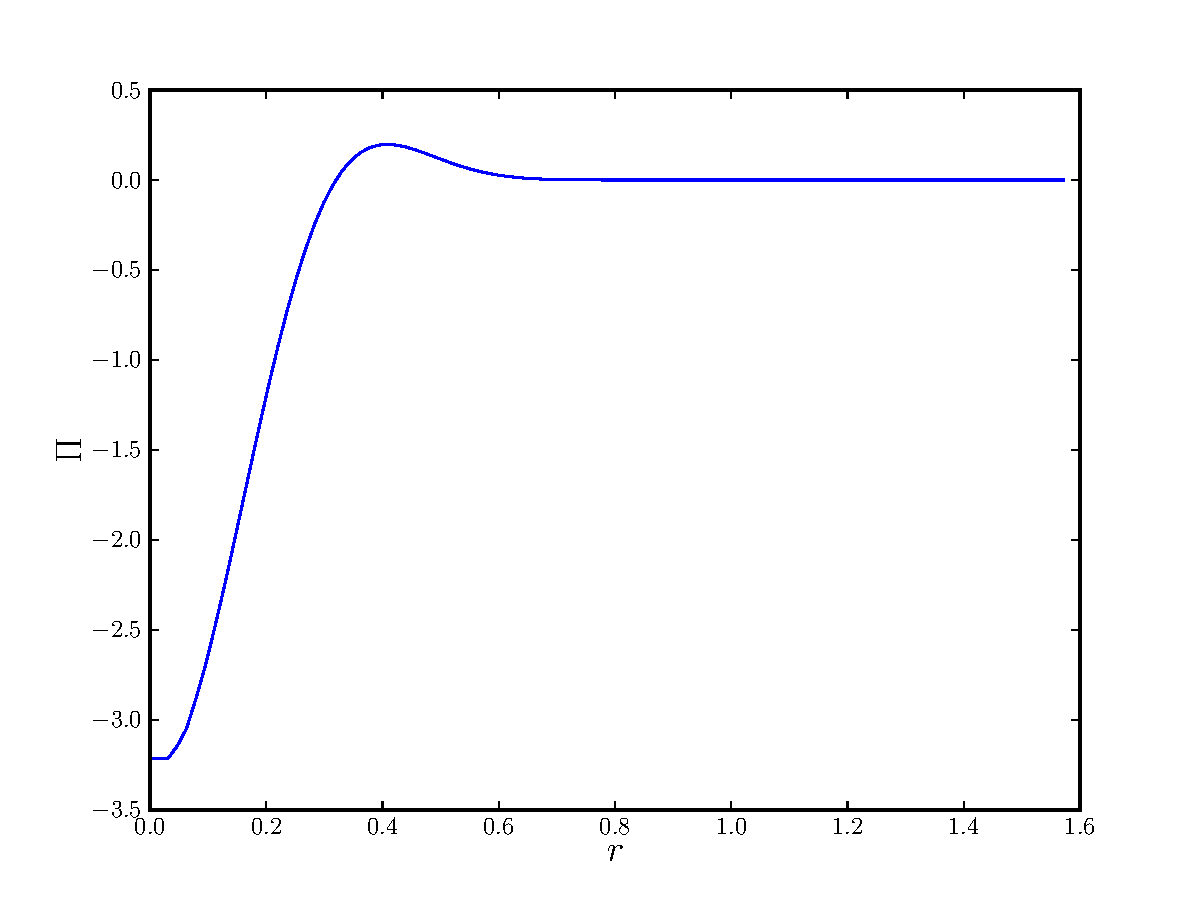
\includegraphics[width=12cm]{./Report/PivrR.pdf}
 \caption{Plot of $\Pi$ vs. r at final time.}
 \label{fig:R-Pi}
\end{figure}

\begin{figure}
 \centering
 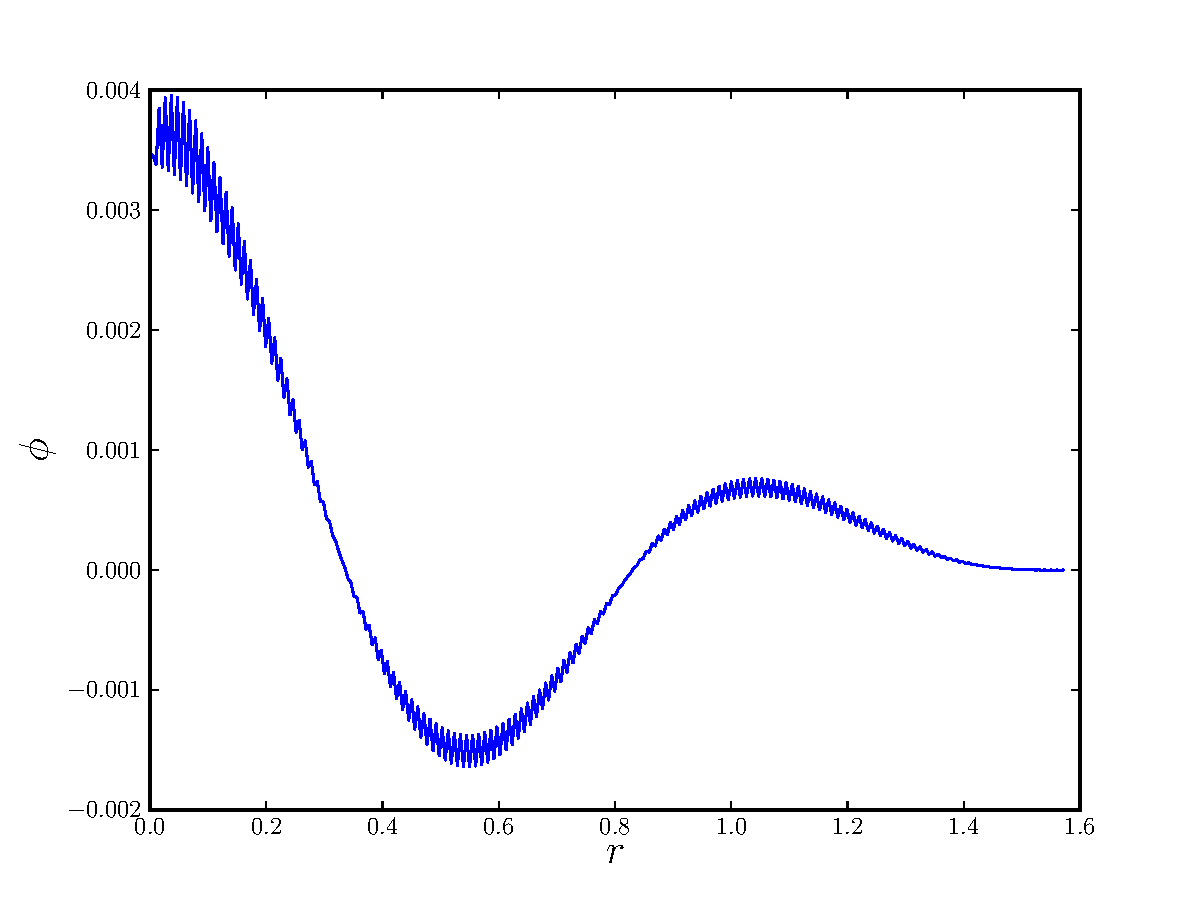
\includegraphics[width=12cm]{./Report/phivrR.pdf}
 \caption{Plot of $\phi$ vs. r at final time.}
 \label{fig:R-phi}
\end{figure}

\begin{figure}
 \centering
 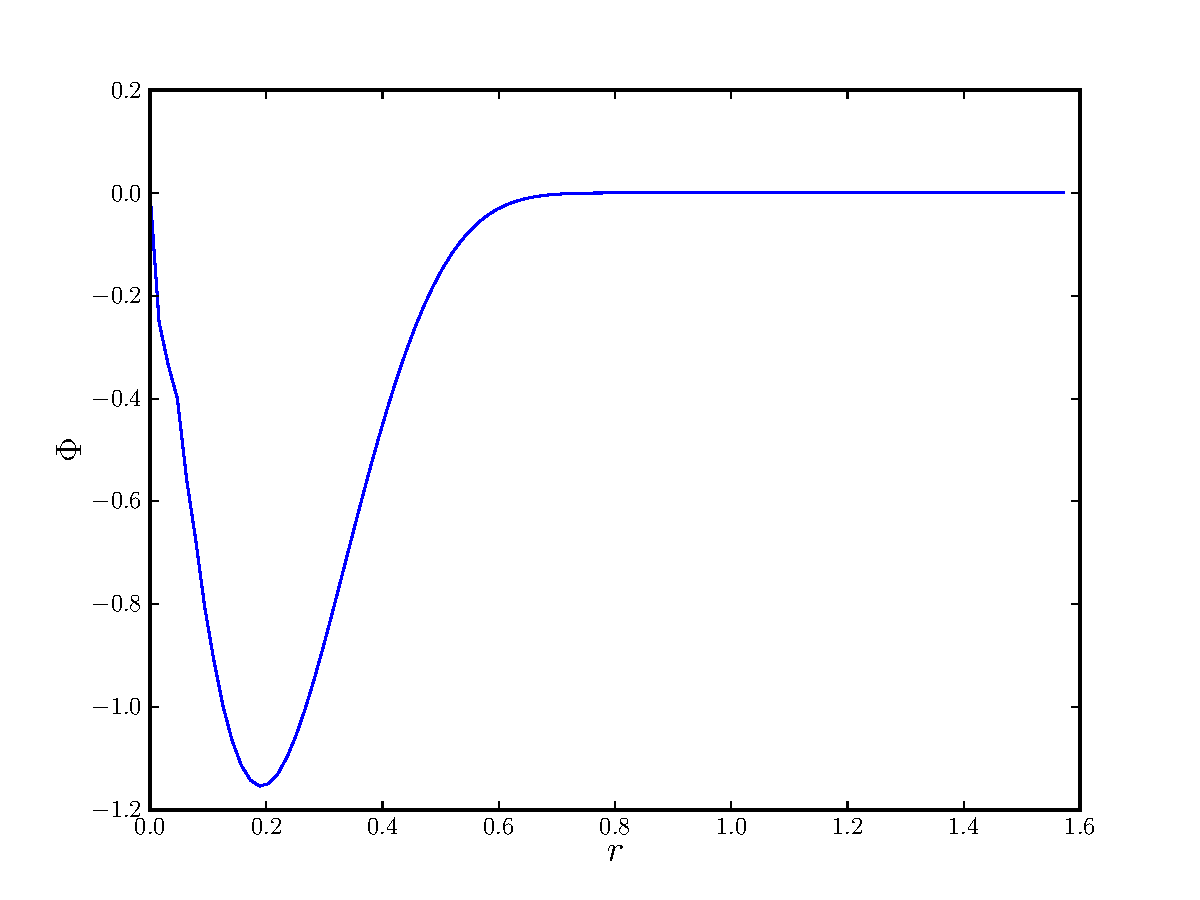
\includegraphics[width=12cm]{./Report/PhivrR.pdf}
 \caption{Plot of $\Phi$ vs. r at final time.}
 \label{fig:R-Phi} 
\end{figure}

\subsection{Black hole formation}

One of the aim of \grv\ is to study the black hole fomration of different fields in \AdS\ geometry. Once the black hole forms the field stops its evolution. It is suggested that all fields forms a black hole at sometimes during their evolution, and it is the universal feature of all fields in \AdS\ . The time of fomation of black hole depends on the amplititude and shape of initial wave, the geometry of space, potential, and the field choice. Because it is not possible to run the code for ever an end condition implimented in the code to stop the evolution of field after some number of iteration. In this run the number of iteration is defined, $i_{\max}  = 1200$. \\
For black hole formation the code checks the value of $A$ at each point, at each time. Theoretically once $A = 0$ it means that the black hole fomed so the condition $A_{\min}$ is defined to check whether the black hole is formed or not. One should choose something close to zero, but independently, by changing the $A_{\min}$ need to make sure that the condition do not affect the result. In this run $A_{\min} = 0.1$ . \\

 In this run the black hole was not formed and the field stoped its evolution at time, $ t = 1.57079632679$. There maybe two resoan why black hole did not form. First the number of iteration was not enough to get the balck hole so by increasing the nuber of iteration once can go furthur in time and see if the black holes forms. Second errors grow and become dominant so the code failed to predict the behavoiur of field. For solving this problem one may want to increase the grid size, in this run grid size of, $n = 300 $, is used. There is another possibilities to improve the numerical solution, change the solver to something more accurate, in this run solver RK4 is used. 

\section{Parameters}

The following parameters are used in this run, \\

Field proparties:
\begin{verbatim}
  Geometry  = AdS4
  Cosmological constant  = 1.0
  Potential = Massive_Scalar
\end{verbatim}

Initial Conditions:
\begin{verbatim}
  Initial Condition = Eigenfunction_modes_non_normalized
\end{verbatim}

Numerical method:
\begin{verbatim}
  Solver = RK4
  Grid size = 300
\end{verbatim}

Ending conditions:
\begin{verbatim}
  Horizon condition (A_min) = 0.1
  Maximum number of iteration = 1200
\end{verbatim}


\section*{ACKNOWLEDGMENTS}
 Arya Farahi wants to thank Andrew Benson for his helpful comments on the code. Arya Farahi wants to thank ... for helping to prepare the tutorial. Also he wants to thank ... for his helpful discussions and ...
 
\end{document}
